\section{The Proposed Solutions}
\subsection{What are the usage data?}

 Program logs contain a wealth of information to help manage systems. Most systems print out program logs during their executions to record system runtime actions and states that can directly reflect system runtime behaviors. System operators usually use these logs to track a system to detect and diagnose system anomalies. However, there are challenges in analyzing program logs in order to understand a system’s behaviors. The program logic of a system usually has a lot of branches, and thus the system’s behaviors may be quite different under different input data or environmental conditions. Knowing the execution behavior under different inputs or configurations can greatly help system operators to understand system behaviors. However, there may be a large number of different combinations of inputs or parameters under different system behaviors. Such complexity poses difficulties for analyzing contextual information related to the state of interest. 

Generally, each log message consists of two different types
of content: a constant string and parameter values. For example, for the first log-printing statement in Table 1, the constant string is “JVM with ID: given task:”, and the printed parameters are JvmId and TaskId. The log messages printed by the same log-print statement contain the same constant string, and are considered to be of the same type, represented by the constant string. 

As summary, there are mainly three sources of usage data can be extracted: the system logs from the cloud services, the application logs, and the logs from the VMs. Fig.~\ref{fig:schema} shows a summary of the three main sources of usage data and the answers for the above questions. The next part of this report, some criteria for the data will be draw and 


\begin{figure}[t!]
	\centering
	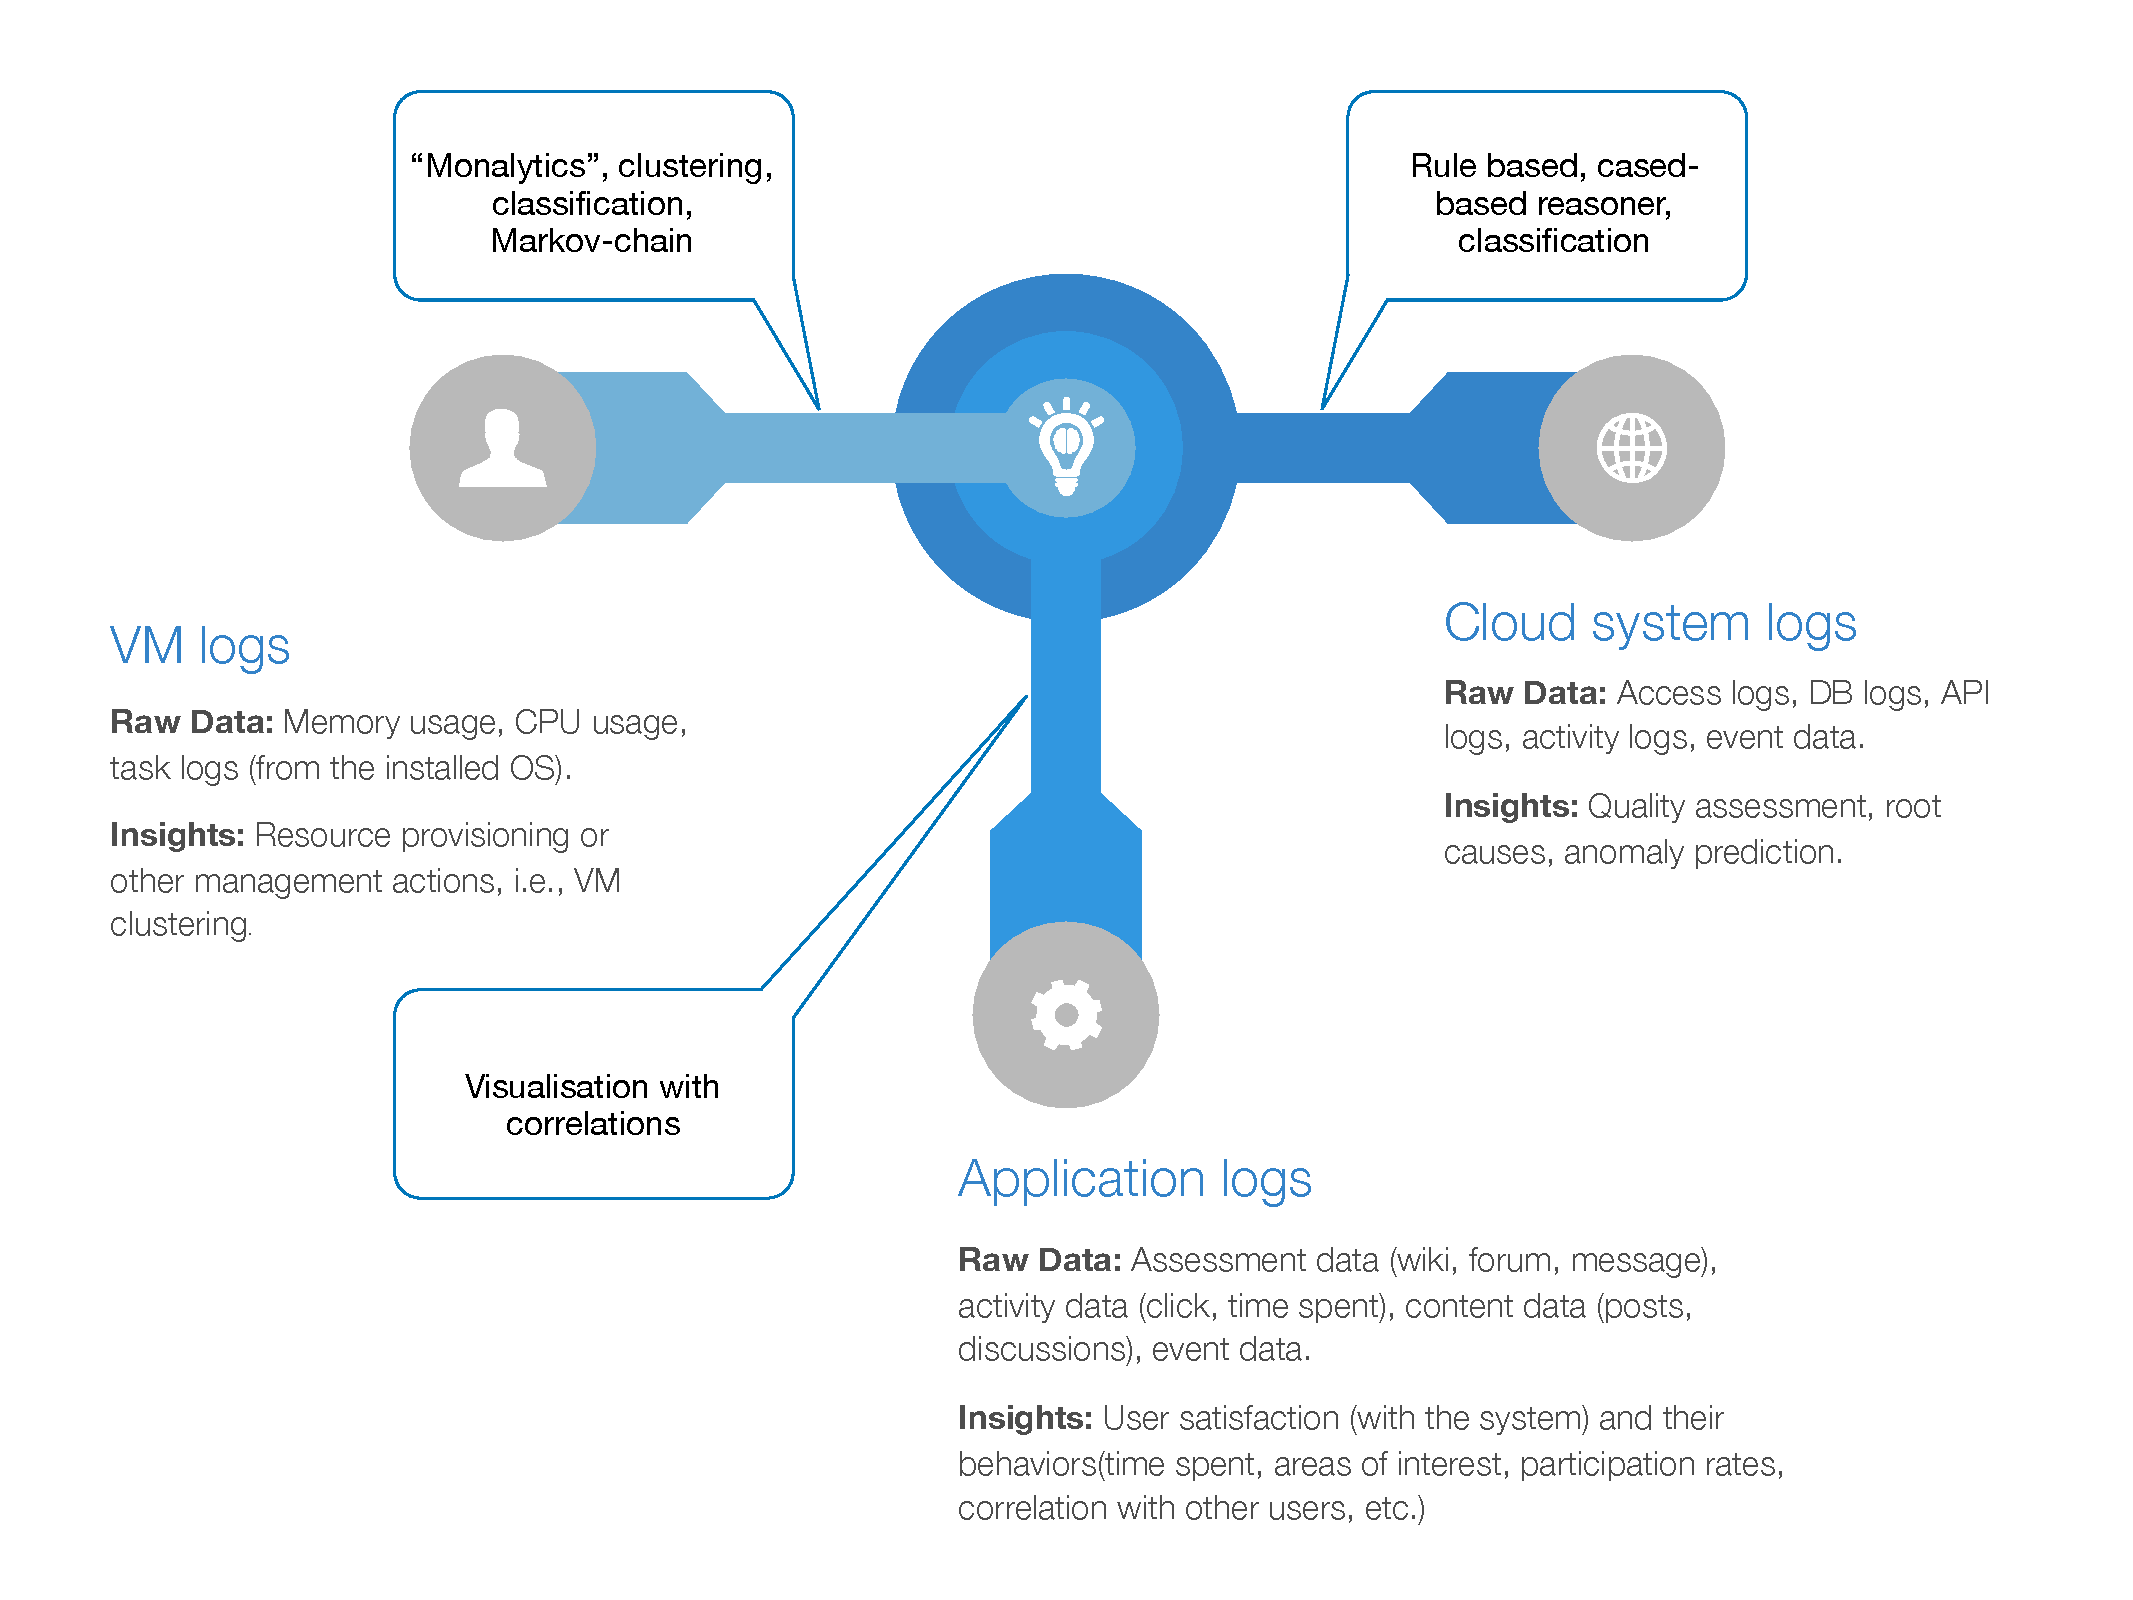
\includegraphics[width=\linewidth]{summary}
	\caption{Three main sources of usage data in cloud-based environment.}
	\label{fig:schema}
\end{figure}



\subsection{Analytics Requirement}

Collecting monitoring data is essential but not suffi- cient per se to explain the observed performance of services. In the next phase, we need to analyze and verify data in light of Service LevelAgreement (SLA) between a customer and a provider. Ideally, the anal- ysis goes beyond simply detecting violation of agreed terms and predicts potential violations. General requirements for an Analytics Engine
(AE) are detailed below. A1. Data Source: AE must be able to fetch moni- toring data recorded in the database. Further, it must be able to query the Cloud middlewares (e.g., that of OpenStack and OpenShift) and application APIs to know the current status of the services. A2. Proactive: AE must support the proactive man- agement of resources. Proactive management needs short term and medium term predictions for the evo-

lution of most relevantmetrics. A3. Alerts: Certain QoS metrics need to be pro- cessed in real time and alerts should be triggered when these QoS metrics are violated or approach cer- tain threshold values. A4. Event Correlation: Detecting the root cause of QoS faults and taking effective counter measures re- quiresmonitoring information spanningmultiple tiers of the virtualized platforms. Quick incomprehensive analysis of monitoring data of individual tiers does not reveal the root cause(s) of the problem precisely enough. Therefore, Analytics need to exhaustively aggregate runtime data from different sources and consolidate information at a high level of abstraction. A5: Identification of Influential Metrics: Identi- fication of the metrics which strongly influence the QoS helps in decreasing the monitoring footprint and analysis complexity.


-------------


Monitoring and Analytic methods have emerged as promising and inevitable solutions in this context, but require precise real time monitoring data. Towards this goal, we assess practical aspects for effective monitoring of SLA-aware services hosted inCloud. We present two real-world application scenarios for deriving requirements and present the prototype of ourMonitoring andAnalytics framework. We claimthat thiswork provides necessary foundations for researching SLA-aware root cause analysis algorithms under realistic setup.

Today more and more (monolithic) applications are decomposed into smaller components which are then executed as services on virtualized platforms con- nected via network communication and orchestrated to deliver the desired functionality. While the foun- dations for decomposing, executing and orchestrat- ing were well settled over the past decade, allocating the needed resources for and steering the execution of components to deliver the requiredQuality of Service (QoS) is an active area of research. A critical aspect of steering complex service-based applications on vir- tualized platforms is effective, non-intrusive, low- footprint monitoring of key performance indicators at different provisioning tiers typically Infrastructure- as-a-Service, Platform-as-a-Service and Software-as- a-Service. These key performance indicators are assessed to verify that a Service Level Agreement (SLA) between a customer and a provider ismet. Ide- ally, the assessment goes beyond simply detecting vi- olations of the agreed terms, but tries to predict and pre-empt potential violations. The provider enacts counter-measures to prevent or resolve the violation if
It it does occur. Deriving effective counter-measures re- quires precise monitoring information spanning mul- tiple tiers of the virtualized platform and analysis of monitoring data to identify the root cause(s) of per- formance problems.

Monitoring systems have been used for decades
in different computing paradigms. Monitoring solu- tions for previous computing paradigms pose signifi- cant limitations for their widespread adoption in large scale, virtual platforms. The major obstacles with these monitoring techniques are, their high perfor- mance overhead, reliability, isolation, limited scala- bility, reliance on proprietary protocols and technolo- gies.

Common performance diagnosis procedures de-
pend on system administrator’s domain knowledge and associated performance best practices. This pro- cedure is labor intensive, error prone, and not feasi- ble for virtual platforms. The prior art on detecting and diagnosing faults in computing systems can be re- viewed in (Appleby et al., 2001) (Molenkamp, 2002) (Agarwal et al., 2004) (Chen et al., 2002)(Barham et al., 2003). These methods do not consider virtual- ization technologies and are inappropriate for rapidly changing, large scale virtual platforms that by very nature require effective automated techniques forQoS fault diagnosis.

Our research motivations are to study the effec-
tiveness and practicality of different techniques for performance problem diagnosis and SLA based re- source management of virtual platforms. This is very well applicable to Cloud Computing where efficient monitoring is essential to accomplish these tasks. The remainder of this paper is organized as follows. Sec- tion 2 presents scenarios of our interest againstwhich in Section 3, we derive requirements for monitoring and analytics. Based on this, in Section 4, we present our Monitoring and Analytics framework prototype developed as part of the GWDG Cloud Infrastructure. Section 5 describes related work and finally, we con- clude the paper in Section 6 with a summary and fu- ture plan.



\section{The Proposed Usage Analytics Methods}

\subsection{Usage Analytics from VM Logs}


\subsection{Usage Analytics from Application Logs}
With the increasing scale and complexity of software
systems, it has become more and more difficult for system operators to understand the behaviors of software systems for tasks such as system problem diagnosis. For example, system operators need to understand system behaviors to figure out why a software system is in the current status. With such an understanding, they can choose the right operations to achieve the desired goal. System behaviors include a series of actions executed by the system and the corresponding changes in the system states. Although operators usually investigate a system starting from a specific state of interest, e.g., a hang state or failure state, contextual information for reaching that state is critical for identifying why the system runs in that state. Such contextual information includes how previous actions are executed by the system, what the historical system states are before running into the state of interest, what the input data is, etc.





2We


\subsection{Usage Analytics from Cloud-based Systems}
	

There are two main categories of challenges to overcome in or-
der to achieve the stated objectives. The first category is rooted from the characteristics of the data being analyzed with analytic technologies. Data scale. Typical data in software analytics is of large scale,
e.g., due to the large scale of software being developed and the large size of software development teams. Some tasks require to analyze division-wide or even company-wide code bases, which are far be- yond the scope of a single code base (e.g., when conducting code- clone detection [2]). Some tasks require to analyze a large quantity of (likely noisy) data samples within or beyond a single code base (e.g., when conducting runtime-trace analysis [3]). Although lack- ing data samples may not be an issue in this context of machine learning, the large scale of data poses challenges for data process- ing and analysis, including learning-algorithm design and system building. Data complexity. Typical data in software analytics is of high
complexity, which is partly due to the high complexity of software being developed. For example, runtime traces fromdistributed sys- tems [3] need to be correlated, while traces frommultiple threads [7] need to be split. System logs [3] include unstructured textual in- formation. There could be high dependencies across traces and noises among traces. In addition, real-world usage data produced from in-field operations offers substantial opportunities for various tasks such as debugging (e.g., those assisted by the Microsoft Er- ror Reporting system [4]). In addition to high complexity, such data is typically distributed and often partial (e.g., collected with sampling-based techniques to reduce runtime overhead). All these characteristics pose challenges for analytic technologies such as machine learning. The second category is rooted from the characteristics of the
tasks being assisted by software analytics. Focus on ultimate tasks being assisted. Among tasks assisted
by software analytics, some tasks are intermediate tasks and some are ultimate tasks. Usually intermediate tasks produce information toward solving ultimate tasks. For example, code-clone detection is considered as an intermediate task, which produces information towards refactoring and defect detection that are ultimate tasks.

Such focus on ultimate tasks requires the mandatory inclusion of the phase of deployment and feedback gathering in the life cycle of a software analytic project. Unlike most previous research on code-clone detection, we should not stop at measuring the preci- sion and recall of detected clones; rather, we should push further to accomplish that the detected clones could effectively help address ultimate tasks such as refactoring and defect detection, and should measure such benefits in evaluations. Engagement of customers during the development process of a
software analytic project. It is well recognized that engaging cus- tomers is a challenging task especially in the context of software engineering tools. Customers may have resistance to proposed changes (due to analytic-tool adoption) on their existing way of carrying out a task. In addition, due to tight development sched- ule, they may not be able to invest time on gaining understanding of the best/worst scenarios for applying an analytic tool. However, developing a software analytic project typically needs the engage- ment of customers in iterations of the four phases in the project life cycle, e.g., to get better understanding on the tasks and domain knowledge. Among the phases, especially the phase of deployment and feedback gathering, it is crucial for the produced analytic tools to have good usability, e.g., providing effective visualization and manipulation of analysis results.